\documentclass[14pt]{article}

\usepackage[utf8]{inputenc}
\usepackage[T2A]{fontenc}
\usepackage[english,russian]{babel}

\usepackage{graphicx}
\usepackage{mathtools,amssymb}
\usepackage{amsmath}

\usepackage{hyperref}

\begin{document}
\section{Постановка задачи}
\begin{figure}
	\center{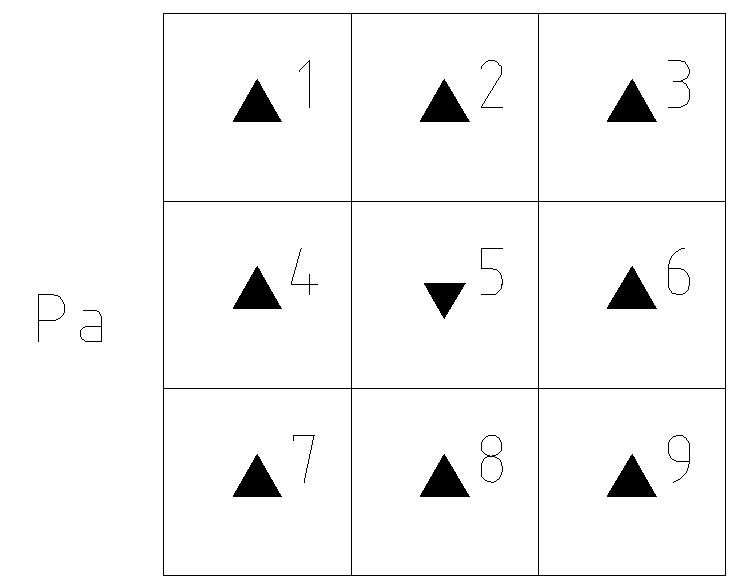
\includegraphics[width=14pc]{1.png}}
	\caption{Схема расчётной области]}
	\label{fig:map}
\end{figure}

	\section{Двухшаговый метод наименьших квадратов}
\begin{equation} \label{fil}
	\triangledown\sigma\triangledown P = \beta^*h\frac{dP}{dt}+\delta(x,y),
\end{equation}

\begin{equation} \label{mape}
	J=\frac{1}{N}\sum_{i=1}^N{\left\vert\frac{p_c^i-p_f^i}{p_f^i}\right\vert},
\end{equation}

\begin{equation} \label{mape}
	f_{_{MAPE}}(x^f,x^c)=\frac{1}{N}\sum_{i=1}^N{\left\vert\frac{x_i^c-x_i^f}{x_i^f}\right\vert},
\end{equation}

\begin{equation} \label{mape}
	J=\sum_{j=1}^M \left( w_j*f_{_{MSE} \ j} \right),
\end{equation}

\begin{equation} \label{mape}
	J=\sum_{j=1}^M \left( w_j*f_{_{MSE} \ j} \right) + \sum_{k=1}^K \left( \alpha_k * f_{pnl \ k}\right),
\end{equation}

	\section{Расчёт погрешности}
	\begin{equation} \label{F_p}
		F'_{p_j} = \sum_{i=1}^N{\frac{dp^c_j}{du_i}}
	\end{equation}
	\begin{equation} \label{F_u}
		F'_{u_j} = \sum_{k=1}^K\sum_{i=1}^N{\frac{dp^c_i}{du_j}\frac{dp^c_i}{du_k}} + 
		\sum_{k=1}^K\sum_{i=1}^N{\frac{d^2p^c_i}{du_j du_k}}
	\end{equation}
	\begin{equation} \label{du_dp}
		\frac{du_i}{dp_j} = \frac{F'_{p_j}}{F'_{u_i}}
	\end{equation}
	\begin{equation} \label{Jf}
		J_f = \frac{1}{N-N_u}\sum_{i=1}^N{\left(p_i^f - p_i^c\right)^2}
	\end{equation}
	\begin{equation} \label{Sp}
		Su = J_f\sqrt{\sum_{i=1}^n{\left(\frac{du_i}{dp^f_j}\right)^2}}
	\end{equation}
	\begin{equation} \label{delta_u}
		\triangle{u} = tp*Su
	\end{equation}
	
	\section{Результаты}
\begin{figure}
	\center{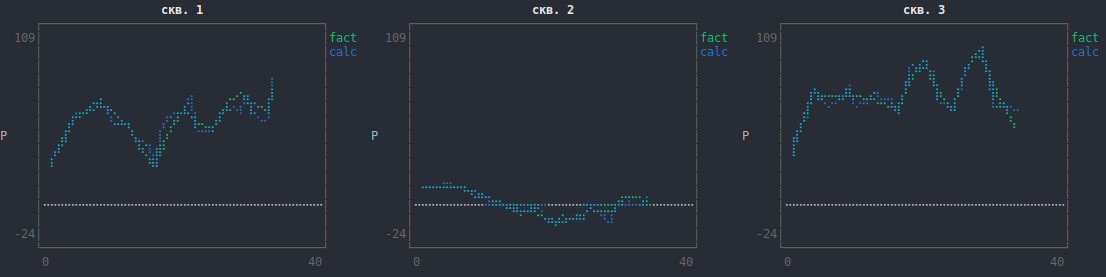
\includegraphics[width=30pc]{1-3.png}}
	\caption{Пластовое давление по скважинам 1-3}
	\label{fig:map}
\end{figure}
\begin{figure}
	\center{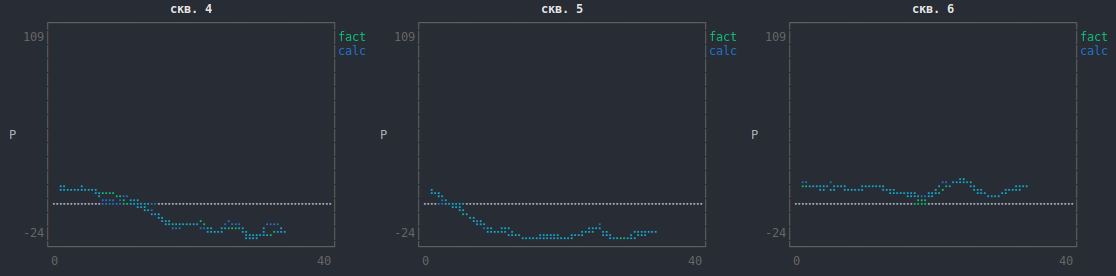
\includegraphics[width=30pc]{4-6.png}}
	\caption{Пластовое давление по скважинам 4-6}
	\label{fig:map}
\end{figure}
\begin{figure}
	\center{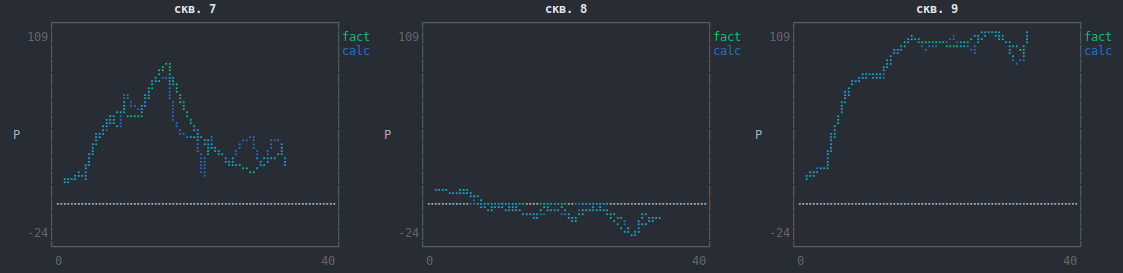
\includegraphics[width=30pc]{7-9.png}}
	\caption{Пластовое давление по скважинам 7-9}
	\label{fig:map}
\end{figure}
метрики по скважинам
\end{document}